\chapter{Снова о многопроцессорности}
\section{Предъявите ваше состояние}
\begin{wrapfigure}{r}{0.35\linewidth}
    
\includegraphics[width=1\linewidth]{turkey.png}
\end{wrapfigure}
Примеры, показанные в предыдущей главе, годились для использования в качестве демонстрационного материала, но с таким ограниченным инструментарием далеко не уйдёшь.
Нет, примеры плохими не назовёшь, но от процессов и акторов пользы мало, когда они представлены только функциями и сообщениями.
Для устранения этого недостатка нам необходимо уметь сохранять в процессе состояние.

Давайте, для начала, создадим функцию в новом модуле \href{http://learnyousomeerlang.com/static/erlang/kitchen.erl}{kitchen.erl}, которая позволит процессу выполнять функции холодильника.
Процессу разрешено совершать две операции: хранить еду в холодильнике и вынимать её оттуда.
Вынимать можно только ту еду, которая была заранее помещена в холодильник.
Пусть основой нашего процесса будет следующая функция:
\begin{lstlisting}[style=erlang]
-module(kitchen).
-compile(export_all).
 
 fridge1() ->
     receive
         {From, {store, _Food}} ->
         From ! {self(), ok},
         fridge1();
     {From, {take, _Food}} ->
         %% uh....
         From ! {self(), not_found},
         fridge1();
     terminate ->
         ok
     end.
\end{lstlisting}

Что\--то здесь не так.
Когда мы делаем запрос на хранение еды, процесс возвращает результат \emph{ok}, но фактически еда нигде не сохраняется.
Будет вызвана функция \emph{fridge1()}, и она начнёт исполняться с чистого листа, без сохранённого состояния.
Очевидно также, что когда мы просим процесс извлечь еду из холодильника, её просто неоткуда взять, и остаётся просто вернуть в качестве результата \emph{not\_found}.
Ясно, что для хранения и извлечения провизии нам необходимо добавить в функцию состояние.

Благодаря рекурсии, состояние процесса может целиком содержаться в параметрах, которые передаются в функцию.
Для нашего процесса\--холодильника можно хранить весь провиант в виде списка, и когда кто\--нибудь захочет поесть, мы сможем поискать в нём необходимый продукт:
\begin{lstlisting}[style=erlang]
fridge2(FoodList) ->
    receive
        {From, {store, Food}} ->
            From ! {self(), ok},
            fridge2([Food|FoodList]);
        {From, {take, Food}} ->
            case lists:member(Food, FoodList) of
                true ->
                    From ! {self(), {ok, Food}},
                    fridge2(lists:delete(Food, FoodList));
                false ->
                    From ! {self(), not_found},
                    fridge2(FoodList)
            end;
        terminate ->
            ok
    end.
\end{lstlisting}

Сразу можно заметить, что \ops{fridge2/1} принимает один аргумент \--- \emph{FoodList}.
Когда мы пошлём сообщение вида \ops{\{From, \{store, Food\}\}} \--- функция добавит значение \emph{Food} в \emph{FoodList} перед следующей итерацией.
На следующей итерации рекурсивного вызова можно будет извлечь из списка тот же самый элемент, который мы туда поместили ранее.
Я даже реализовал эту возможность.
Функция использует \ops{lists:member/2} для проверки наличия \ops{Food} в \ops{FoodList}.
В зависимости от результата, полученный элемент либо пересылается вызывающему процессу (и удаляется из \emph{FoodList}), либо получателю отсылается атом \emph{not\_found}:
\begin{lstlisting}[style=erlang]
1> c(kitchen).
{ok,kitchen}
2> Pid = spawn(kitchen, fridge2, [[baking_soda]]).
<0.51.0>
3> Pid ! {self(), {store, milk}}.
{<0.33.0>,{store,milk}}
4> flush().
Shell got {<0.51.0>,ok}
ok
\end{lstlisting}

Функция хранения продуктов в холодильнике вроде бы работает.
Теперь попробуем поместить туда различные продукты, а затем их извлечь.
\begin{lstlisting}[style=erlang]
5> Pid ! {self(), {store, bacon}}.
{<0.33.0>,{store,bacon}}
6> Pid ! {self(), {take, bacon}}.
{<0.33.0>,{take,bacon}}
7> Pid ! {self(), {take, turkey}}.
{<0.33.0>,{take,turkey}}
8> flush().
Shell got {<0.51.0>,ok}
Shell got {<0.51.0>,{ok,bacon}}
Shell got {<0.51.0>,not_found}
ok
\end{lstlisting}

В соответствии с нашими ожиданиями, мы можем достать из холодильника бекон, потому что мы его туда поместили первым по счёту (вместе с молоком и пищевой содой), но когда мы просим процесс\--холодильник достать немного мяса индейки, у него ничего не выходит.
Именно поэтому мы получаем последнее сообщение \ops{\{<0.51.0>,not\_found\}}.
\section{Мы любим послания, но держим их в секрете}
\label{we-love-messages-but-we-keep-them-secret}
В предыдущем примере немного раздражает то, что программист, который собирается воспользоваться холодильником, должен иметь представление о протоколе, который был изобретён специально для этого процесса.
Что ведёт к усложнению без видимой на то необходимости.
Этот недостаток можно устранить, абстрагируя сообщения при помощи функций, которые эти сообщения получают и отправляют:
\begin{lstlisting}[style=erlang]
store(Pid, Food) ->
    Pid ! {self(), {store, Food}},
    receive
        {Pid, Msg} -> Msg
    end.
 
take(Pid, Food) ->
    Pid ! {self(), {take, Food}},
    receive
        {Pid, Msg} -> Msg
    end.
\end{lstlisting}

В таком виде взаимодействие с процессом выглядит гораздо опрятнее:
\begin{lstlisting}[style=erlang]
9> c(kitchen).
{ok,kitchen}
10> f().
ok
11> Pid = spawn(kitchen, fridge2, [[baking_soda]]).
<0.73.0>
12> kitchen:store(Pid, water).
ok
13> kitchen:take(Pid, water).
{ok,water}
14> kitchen:take(Pid, juice).
not_found
\end{lstlisting}

Нам больше не нужно переживать о том, как в принципе работают сообщения, нужно ли нам посылать \ops{self()} или какой\--то конкретный атом из числа \ops{take} или \ops{store}.
Мы должны знать лишь pid и то, какую функцию нужно вызвать.
Это позволяет спрятать подальше от глаз всю грязную работу и облегчает создание процесса\--холодильника.

Осталось только спрятать саму необходимость порождения процесса.
Мы позаботились о сокрытии сообщений, но обязанности по созданию процесса мы возложили на программиста.
Я добавлю следующую функцию \ops{start/1}:
\begin{lstlisting}[style=erlang]
start(FoodList) ->
    spawn(?MODULE, fridge2, [FoodList]).
\end{lstlisting}

\begin{wrapfigure}{r}{0.5\linewidth}
    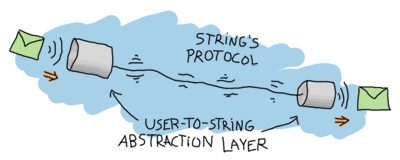
\includegraphics[width=1\linewidth]{abstraction.png}
\end{wrapfigure}
\ops{?MODULE} \--- это макрос, который возвращает имя текущего модуля.
Казалось бы, запись такой функции не несёт никаких преимуществ, но на самом деле некоторые преимущества есть.
Самым главным из них является согласованность с вызовами функций \ops{take/2} и \ops{store/2}.
Все операции процесса\--холодильника теперь обрабатываются модулем \href{http://learnyousomeerlang.com/static/erlang/kitchen.erl}{kitchen}.
Если вам необходимо добавить запись о времени старта процесса\--холодильника, или запустить второй процесс (к примеру, морозильник), то это можно легко сделать внутри нашей функции \ops{start/1}.
Но если порождение процесса будет делать пользователь при помощи \ops{spawn/3}, то в каждом месте, где запускается холодильник, мы будем обязаны добавить вызовы новых функций.
Здесь очень просто совершить ошибку, а ошибки это плохо.

Взглянем на эту функцию в деле:
\begin{lstlisting}[style=erlang]
15> f().
ok
16> c(kitchen).
{ok,kitchen}
17> Pid = kitchen:start([rhubarb, dog, hotdog]).
<0.84.0>
18> kitchen:take(Pid, dog).
{ok,dog}
19> kitchen:take(Pid, dog).
not_found
\end{lstlisting}

Ура!
Собака выбралась из холодильника, и наша абстракция готова к использованию!
\section{Тайм\--аут}
\label{time-out}
Давайте попробуем сделать кое\--что при помощи команды \ops{pid(A,B,C)}, которая позволяет нам преобразовать 3 целых числа \emph{A}, \emph{B} и \emph{C} в pid.
Попробуем намеренно передать функции \ops{kitchen:take/2} несуществующий pid:
\begin{lstlisting}[style=erlang]
20> kitchen:take(pid(0,250,0), dog).
\end{lstlisting}

Ой, оболочка зависла.
Зависание было вызвано реализацией функции \ops{take/2}.
Попробуем разобраться в произошедшем, и для начала рассмотрим события, которые происходят в случае нормального выполнения:
\begin{enumerate}
    \item От вас (от оболочки) пересылается сообщение процессу\--холодильнику, с указанием сохранить еду;
    \item Ваш процесс переключается в режим приёма и ожидает появления нового сообщения;
    \item Холодильник сохраняет элемент и посылает вашем процессу сообщение 'ok';
    \item Ваш процесс получает это подтверждение и продолжает заниматься своими делами.
\end{enumerate}
А вот что происходит при зависании оболочки:
\begin{enumerate}
    \item От вас (от оболочки) к неизвестному процессу уходит сообщение с указанием сохранить еду;
    \item Ваш процесс переключается в режим приёма и ожидает новое сообщение;
    \item Неизвестный процесс не существует вовсе, либо не ожидает получить ваше сообщение, и после его получения ничего с ним не делает;
    \item Процесс вашей оболочки застревает в режиме приёма.
\end{enumerate}
\begin{wrapfigure}{r}{0.15\linewidth}
    
\includegraphics[width=1\linewidth]{hourglass.png}
\end{wrapfigure}

Досадно, особенно если учесть, что эту ошибку нельзя обработать.
Ничего плохого не происходит, программа просто находится в режиме ожидания.
Как правило, любой код, имеющий дело с асинхронными операциями (а именно так организована передача сообщений в Erlang), должен иметь возможность прекращать ожидание по прошествии некоторого времени, если информация так и не была получена.
Похожую операцию проделывает веб\--браузер, когда загрузка страницы или изображения продолжается слишком долго.
Вы и сами проделываете то же самое, если при совершеннии телефонного звонка абонент долго не берёт трубку, или когда кто\--то не приходит на встречу вовремя.
Само собой, в Erlang на этот случай имеется соответствующий механизм, который является частью конструкции \ops{receive}.
\begin{lstlisting}[style=erlang]
receive
    Match -> Expression1
after Delay ->
    Expression2
end.
\end{lstlisting}

За выполнение того, о чём мы только что говорили, отвечает часть кода, которая находится между \ops{receive} и \ops{after}.
Код в \ops{after} будет выполнен, если за время равное \emph{Delay} (целое значение, заданное в миллисекундах) не будет получено сообщение, которое соответствует шаблону \emph{Match}.
В этом случае выполняется \emph{Expression2}.

Напишем пару новых функций интерфейса \ops{store2/2} и \ops{take2/2}, которые будут вести себя абсолютно так же как \ops{store/2} и \ops{take/2}, но прекращать ожидание после 3\--х секунд:
\begin{lstlisting}[style=erlang]
store2(Pid, Food) ->
    Pid ! {self(), {store, Food}},
    receive
        {Pid, Msg} -> Msg
    after 3000 ->
        timeout
    end.
 
take2(Pid, Food) ->
    Pid ! {self(), {take, Food}},
    receive
        {Pid, Msg} -> Msg
    after 3000 ->
        timeout
    end.
\end{lstlisting}

Теперь вы можете вывести оболочку из зависшего состояния нажатием Ctrl-G, и испытать новые интерфейсные функции:
\begin{lstlisting}[style=erlang]
User switch command
 --> k
 --> s
 --> c
Eshell V5.7.5  (abort with ^G)
1> c(kitchen).
{ok,kitchen}
2> kitchen:take2(pid(0,250,0), dog).
timeout
\end{lstlisting}

Вот теперь всё работает.\\
\colorbox{lgray}
{
\begin{minipage}{1.0\linewidth}
    \textbf{Замечание:} я говорил, что \ops{after} принимает значения только в миллисекундах, но ему также можно передавать атом \ops{infinity}.
    Во многих случаях от этой возможности мало проку (тогда выражение \ops{after} можно было бы полностью удалить), но иногда её используют, если программист имеет возможность передать время ожидания в функцию, в которой предполагается получение результата.
    Ожидание в такой ситуации действительно может продолжаться вечно, если этого захочет программист.
\end{minipage}
}

Кроме случаев, когда нужно прекращать слишком долгое ожидание, такие таймеры могут пригодиться и в других ситуациях.
Простым примером может послужить то, как работает функция \ops{\href{http://erldocs.com/R15B/timer.html\#sleep/1}{time:sleep/1}}, которую мы использовали ранее.
Вот как она реализована (поместим её в новый модуль \href{http://learnyousomeerlang.com/static/erlang/multiproc.erl}{multiproc.erl}):
\begin{lstlisting}[style=erlang]
sleep(T) ->
    receive
    after T -> ok
    end.
\end{lstlisting}

В \ops{receive} не будет найдено совпадение ни с одним из сообщений, так как для сопоставления не задан шаблон.
По истечении периода \emph{T} будет просто выполнена \ops{after} часть конструкции.

А вот ещё один особый случай, когда таймаут равен 0:
\begin{lstlisting}[style=erlang]
flush() ->
    receive
        _ -> flush()
    after 0 ->
        ok
    end.
\end{lstlisting}

В такой ситуации виртуальная машина Erlang будет пытаться найти сообщение, совпадающе с одним из указанных шаблонов.
В вышеприведённом случае подойдёт что угодно.
Функция \ops{flush/0} будет рекурсивно себя вызывать, пока в почтовом ящике есть сообщения, до полного их исчерпания.
Когда ящик окажется пуст, выполнится код \ops{after 0 -> ok} и функция завершит выполнение.
